\section{大富翁游戏的概率}\label{sec:problem84}
\subsection{问题描述}
\begin{tcolorbox}[breakable]

	在经典的英国版\enquote{大富翁}(Monopoly)游戏中,棋盘由以下顺序的方格组成:

	\begin{center}
		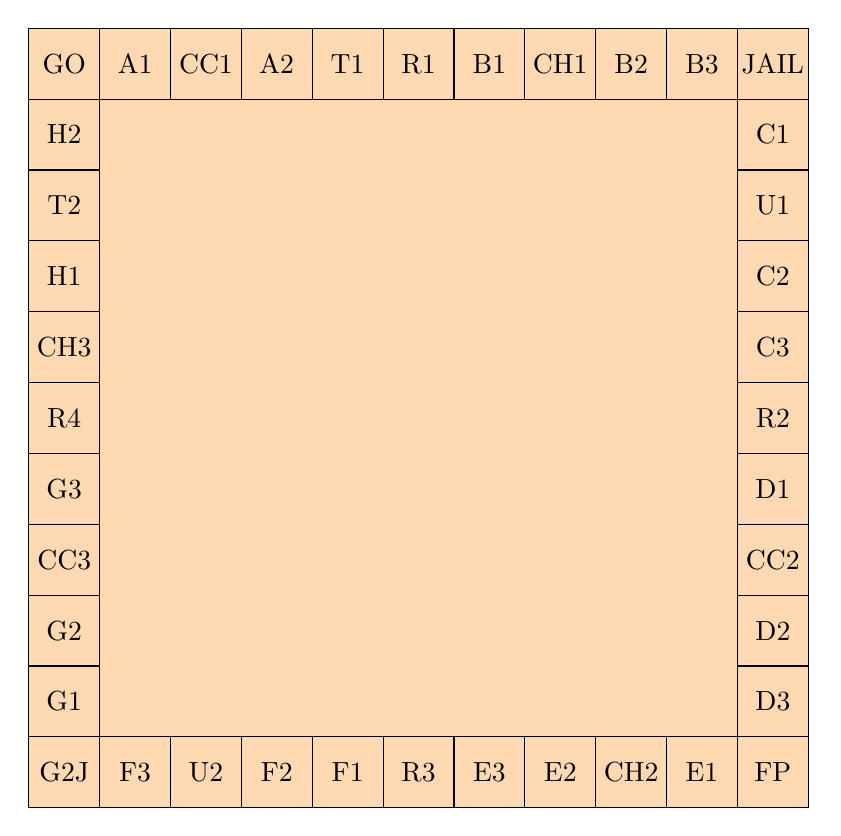
\begin{tikzpicture}[scale=0.6]
			\def\cellwidth{1.5cm}
			\def\cellheight{1.5cm}

			% Colors
			\fill[orange!30] (0, 0) rectangle (11*\cellwidth, 11*\cellheight);

			% Board cells
			\foreach \i in {0,...,10} {
					% Bottom row
					\draw (\i*\cellwidth, 0) rectangle ++(\cellwidth, \cellheight);

					% Top row
					\draw (\i*\cellwidth, 10*\cellheight) rectangle ++(\cellwidth, \cellheight);

					% Left column
					\draw (0, \i*\cellheight) rectangle ++(\cellwidth, \cellheight);

					% Right column
					\draw (10*\cellwidth, \i*\cellheight) rectangle ++(\cellwidth, \cellheight);
				}

			% Bottom row labels
			\node at (0.5*\cellwidth, 0.5*\cellheight) {G2J};
			\node at (1.5*\cellwidth, 0.5*\cellheight) {F3};
			\node at (2.5*\cellwidth, 0.5*\cellheight) {U2};
			\node at (3.5*\cellwidth, 0.5*\cellheight) {F2};
			\node at (4.5*\cellwidth, 0.5*\cellheight) {F1};
			\node at (5.5*\cellwidth, 0.5*\cellheight) {R3};
			\node at (6.5*\cellwidth, 0.5*\cellheight) {E3};
			\node at (7.5*\cellwidth, 0.5*\cellheight) {E2};
			\node at (8.5*\cellwidth, 0.5*\cellheight) {CH2};
			\node at (9.5*\cellwidth, 0.5*\cellheight) {E1};
			\node at (10.5*\cellwidth, 0.5*\cellheight) {FP};

			% Left column labels
			\node at (0.5*\cellwidth, 1.5*\cellheight) {G1};
			\node at (0.5*\cellwidth, 2.5*\cellheight) {G2};
			\node at (0.5*\cellwidth, 3.5*\cellheight) {CC3};
			\node at (0.5*\cellwidth, 4.5*\cellheight) {G3};
			\node at (0.5*\cellwidth, 5.5*\cellheight) {R4};
			\node at (0.5*\cellwidth, 6.5*\cellheight) {CH3};
			\node at (0.5*\cellwidth, 7.5*\cellheight) {H1};
			\node at (0.5*\cellwidth, 8.5*\cellheight) {T2};
			\node at (0.5*\cellwidth, 9.5*\cellheight) {H2};
			\node at (0.5*\cellwidth, 10.5*\cellheight) {GO};

			% Top row labels
			\node at (1.5*\cellwidth, 10.5*\cellheight) {A1};
			\node at (2.5*\cellwidth, 10.5*\cellheight) {CC1};
			\node at (3.5*\cellwidth, 10.5*\cellheight) {A2};
			\node at (4.5*\cellwidth, 10.5*\cellheight) {T1};
			\node at (5.5*\cellwidth, 10.5*\cellheight) {R1};
			\node at (6.5*\cellwidth, 10.5*\cellheight) {B1};
			\node at (7.5*\cellwidth, 10.5*\cellheight) {CH1};
			\node at (8.5*\cellwidth, 10.5*\cellheight) {B2};
			\node at (9.5*\cellwidth, 10.5*\cellheight) {B3};
			\node at (10.5*\cellwidth, 10.5*\cellheight) {JAIL};

			% Right column labels
			\node at (10.5*\cellwidth, 9.5*\cellheight) {C1};
			\node at (10.5*\cellwidth, 8.5*\cellheight) {U1};
			\node at (10.5*\cellwidth, 7.5*\cellheight) {C2};
			\node at (10.5*\cellwidth, 6.5*\cellheight) {C3};
			\node at (10.5*\cellwidth, 5.5*\cellheight) {R2};
			\node at (10.5*\cellwidth, 4.5*\cellheight) {D1};
			\node at (10.5*\cellwidth, 3.5*\cellheight) {CC2};
			\node at (10.5*\cellwidth, 2.5*\cellheight) {D2};
			\node at (10.5*\cellwidth, 1.5*\cellheight) {D3};

		\end{tikzpicture}
	\end{center}
	玩家从\enquote{GO}方格开始,掷两颗六面骰,点数之和决定顺时针前进的步数。如果没有其他规则的影响,每个方格的访问概率应为均等的2.5\%。然而,落在\enquote{G2J}(Go To Jail)、\enquote{CC}(Community Chest,社区基金)和\enquote{CH}(Chance,机会)等方格会改变这种分布。此外,如果玩家连续掷出三次双骰(即两颗骰子点数相同),他们不会根据第三次掷骰的结果前进,而是直接进入监狱。

	在游戏开始时,\enquote{CC}和\enquote{CH}牌堆会被洗牌。当玩家落在\enquote{CC}或\enquote{CH}方格时,他们从相应的牌堆顶部抽取一张牌,按照指示执行后,将牌放回牌堆底部。每个牌堆各有16张牌,但在本题中,我们只关注那些指示玩家移动的牌;其他不涉及移动的指示将被忽略,玩家仍留在原方格。

	社区基金(CC)牌堆中的移动指令(2/16张):

	\begin{itemize}
		\item 	前进至\enquote{GO}
		\item 	直接进入监狱
	\end{itemize}

	机会(CH)牌堆中的移动指令(10/16张):
	\begin{itemize}
		\item 	前进至\enquote{GO}
		\item 	直接进入监狱
		\item 	前进至\enquote{C1}
		\item 	前进至\enquote{E3}
		\item 	前进至\enquote{H2}
		\item 	前进至\enquote{R1}
		\item 	前进至下一个铁路公司(R)
		\item 	前进至下一个铁路公司(R)
		\item 	前进至下一个公用事业公司(U)
		\item 	后退3格
	\end{itemize}

	本题的核心在于计算玩家落在特定方格的概率,即每次掷骰后最终停留在该方格的概率。因此,除了\enquote{G2J}方格(其最终停留概率为0)外,\enquote{CH}方格的概率应最低,因为有5/8的概率会指示玩家移动到其他方格。我们关注的是每次掷骰后玩家最终停留的方格。

	我们将不区分\enquote{只是参观}(Just Visiting)和被送入监狱的状态,也忽略\enquote{出狱}时需要掷出双骰的规则,假设玩家在下一回合支付罚款出狱。

	从\enquote{GO}开始,将格按顺序编号为00到39,我们可以将这些两位数的编号连接起来,形成对应方格的字符串。统计显示,访问概率最高的三个方格依次是:监狱(6.24\%)= 方格10,E3(3.18\%)= 方格24,和GO(3.09\%)= 方格00。因此,这三个最常被访问的方格可以用六位数的字符串表示为:102400。

	如果改用两颗四面骰,求访问概率最高的三个方格,并用六位数的字符串表示。

\end{tcolorbox}

\subsection{算法}

\subsection{答案}
